\documentclass{article}
\usepackage{amsmath}
\usepackage{graphicx}
\usepackage{geometry}
\usepackage{parskip}

\geometry{margin=1in}

\begin{document}

\title{Task 1 Summary}
\author{Jonas Alber (), Schweitzer Tim (29844429)}
\date{November 9, 2024}

\maketitle 

\section*{Overview}
This document provides an explanation of the process used for augmented reality (AR) rendering with Aruco markers.

\section*{Steps in the Process}
\subsection*{1. Loading the Images}
Two images are loaded into memory using the OpenCV \texttt{cv2.imread} function:
\begin{itemize}
    \item The base image containing the Aruco markers.
    \item The poster image to be overlaid on the detected markers.
\end{itemize}

\subsection*{2. Aruco Marker Detection}
Aruco markers are detected using \texttt{cv2.aruco.detectMarkers}, which:
\begin{itemize}
    \item Uses a predefined dictionary (\texttt{DICT\_6X6\_250}) to match marker patterns.
    \item Returns the coordinates of detected marker corners.
\end{itemize}
The output is essential for aligning the AR content with the physical markers in the base image.

\subsection*{3. Perspective Transformation}
The function \texttt{cv2.getPerspectiveTransform} calculates a perspective transformation matrix (\textit{M}) by mapping the scaled coordinates of the poster to the detected marker coordinates. This step ensures that the AR content aligns correctly, compensating for the viewpoint distortion of the camera.

\begin{figure}[h]
    \centering
    \includegraphics[width=0.7\textwidth]{transformed_poster.png}
    \caption{Poster transformed to match the perspective of the Aruco marker.}
\end{figure}

\subsection*{4. Mask Creation and Application}
To prepare for overlay:
\begin{itemize}
    \item A mask is created using \texttt{cv2.fillPoly} to define the overlay area.
    \item The mask is inverted (\texttt{cv2.bitwise\_not}) to retain parts of the original image outside the overlay area.
    \item A bitwise AND operation (\texttt{cv2.bitwise\_and}) removes the overlay region from the base image.
\end{itemize}
This step clears the AR region for the poster while preserving the rest of the base image.

\begin{figure}[h]
    \centering
    \includegraphics[width=0.7\textwidth]{mask.png}
    \caption{Binary mask defining the overlay region.}
\end{figure}

\subsection*{5. Overlaying the Transformed Poster}
The resized and transformed poster is added to the cleared region using a bitwise OR operation (\texttt{cv2.bitwise\_or}). An optional border (\texttt{cv2.polylines}) can be drawn around the overlay area for emphasis.

\begin{figure}[h]
    \centering
    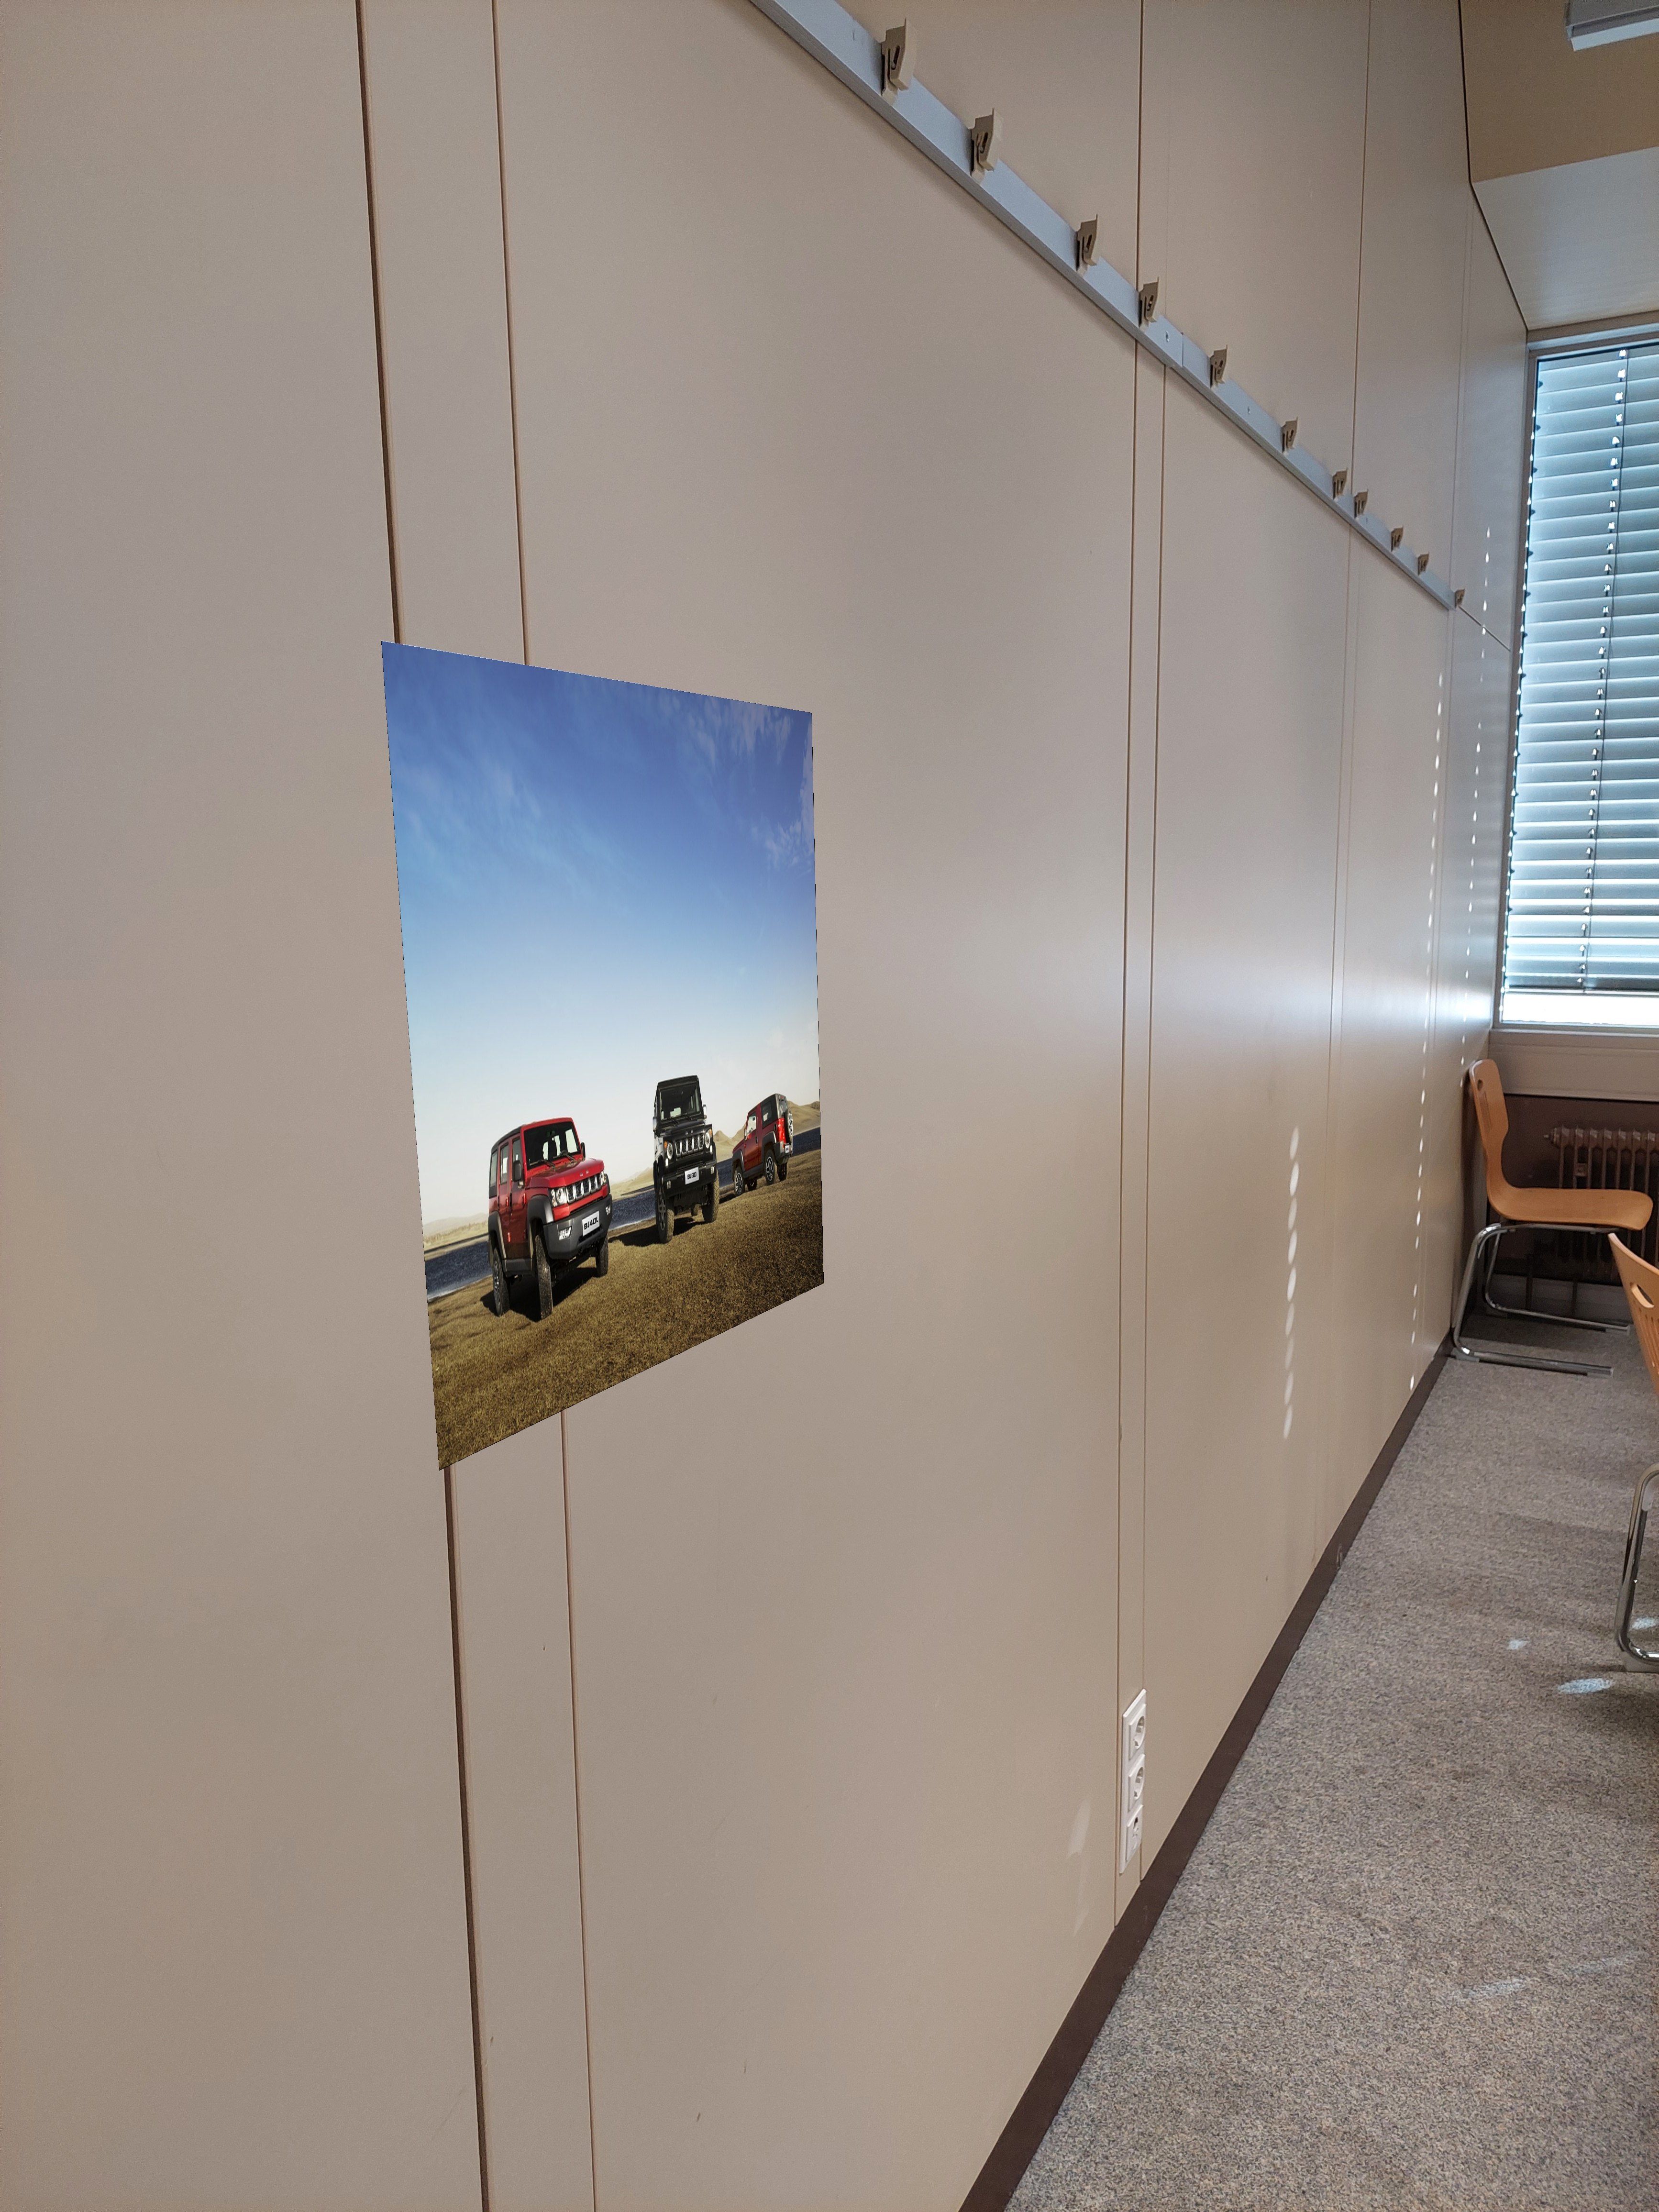
\includegraphics[width=0.7\textwidth]{20221115_113440.png}
    \caption{Final image with the transformed poster overlaid.}
\end{figure}

\section*{Challenges and Potential Improvements}
\subsection*{Challenges}
\begin{itemize}
    \item \textbf{Scaling Issues:} If the detected marker is small compared to the poster size, distortions may arise.
    \item \textbf{Single Marker Limitation:} Relying on a single marker can limit the stability and accuracy of the AR effect, especially for larger overlays.
\end{itemize}

\subsection*{Improvements and Limitations}
\begin{itemize}
    \item \textbf{Using Multiple Markers:} Adding multiple Aruco markers can enhance the precision of the overlay and better define the area for the AR content.
    \item \textbf{Camera Calibration:} Implementing pose estimation with a calibrated camera could improve alignment accuracy, especially in real-world applications.
    \item \textbf{Limitations:} These improvements were not implemented in the current version due to the limitations set by the Project.
\end{itemize}

\section*{Conclusion}
This project demonstrates how Aruco markers and OpenCV can be used for augmented reality overlays. The workflow incorporates marker detection, perspective transformation, masking, and bitwise operations to achieve an accurate AR effect. While effective, in some cases the errors in scaling and placing become very clear.

\end{document}
